\documentclass[12pt,a4paper]{article}
\usepackage{preamble}
\usepackage{graphicx}
\usepackage{fancyvrb}
\newcommand\sessiontitle{Lab Session 3}
\newcommand\sessionsubtitle{Mean, Median, and Gaussian filtering}

%%%%%%%%%%%%%%%%%%%%%%%%%%%%%%%%%%%%%%%%%%
\begin{document}

\paragraph{Preparation.} Open the notebook \texttt{task3.ipynb} in VS Code (see Task 2 of Lab Session 1). Enter the ``\texttt{import numpy}'' and ``\texttt{import matplotlib.pyplot as plt}'' instructions into the \emph{first} code cell of the notebook and run it (cf.\ Lab Session~2).

\section{Linear filtering by convolution (mean filter)}
\label{task:boxfilter}
In this task you will implement and test a \emph{mean filter} (box filter).
\begin{enumerate}
    \item Use \texttt{imread} and \texttt{imshow} to load and show the image \texttt{data/lena.png}.
    \item Finish the implementation of the re-usable function \texttt{meanfilter}. The function parameters are \texttt{img} (the image to be filtered) and \texttt{size} (filter size determining the filtering neighborhood). You may assume that \texttt{size} is an odd number. The function must return the filtered result image. Do \emph{not} modify the input image \texttt{img}!
    \item Test your solution by using the function \texttt{meanfilter} for the previously loaded image (e.g., set the filter size to \texttt{3}). If something does not work as expected, look for errors you have made and fix them. Repeat fixing and testing until everything works.
    \item Compare your result for filter size \texttt{5} with the correct result image \texttt{data/lena\_mean\-fil\-ter5.png}. Use \texttt{imread} to load the image. For a \emph{quantitative} comparison of two images, use the instruction ``\texttt{assert numpy.allclose(img1, img2, atol=1/255)}'' where ``\texttt{img1}'' and ``\texttt{img2}'' are the two images -- \textbf{Notes:}
    \begin{enumerate}
        \item The instruction ``\texttt{assert condition}'' interrupts the code execution if \texttt{condition} is \texttt{False}, rising your attention to an error. Otherwise, nothing happens.
        \item In contrast to a comparison using the mathematical equality operator (``\texttt{img1 == img2}''), a comparison using \texttt{allclose} tolerates \emph{numerical inaccuracies}. The parameter ``\texttt{atol=1/255}'' specifies the maximum tolerated difference per pixel. Since the PNG file quantifies image intensities as multiples of $1/255$, errors lower than $1/255$ cannot be distinguished from numerical inaccuracies.
    \end{enumerate}
\end{enumerate}

\noindent\textbf{Hints:}
\begin{enumerate}
    \item To create a new \texttt{numpy.ndarray} object representing an image with height \texttt{shape[0]} and width \texttt{shape[1]}, initially filled with zeros, you can use \texttt{numpy.zeros(shape)}.
    \item You can use two nested \texttt{for}-loops: An \emph{outer} \texttt{for}-loop to iterate over all pixels of the image and an \emph{inner} \texttt{for}-loop to iterate over all pixels of the filtering neighborhood.
    \item To iterate over all pixels of the image or the filtering neighborhood using a \texttt{for}-loop, \texttt{ndindex} can be used (cf.\ Lab Session~2, Task~3.2(b)).
    \item Bear in mind the border problem, i.e.\ you should not access pixels where the neighborhood is partially outside the image.
    \item Also consider the schematic illustration in Figure~\ref{fig:filtering_neighborhood}.
\end{enumerate}
\begin{figure}[h!]
    \centering
    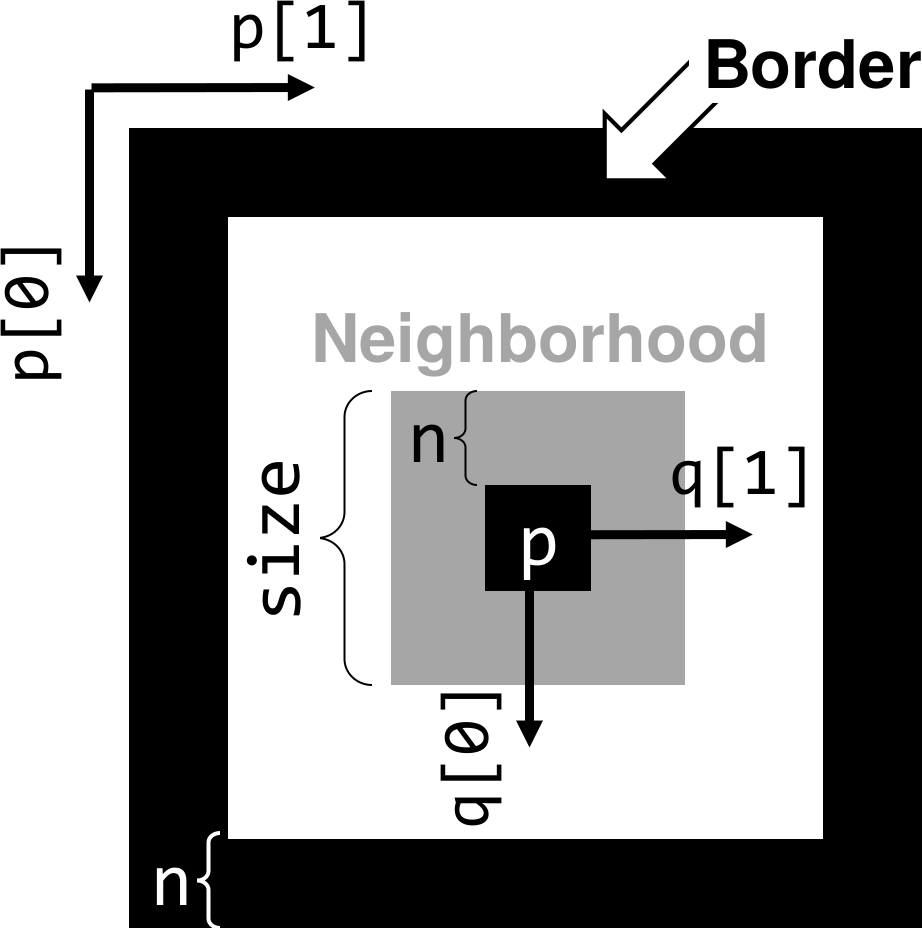
\includegraphics[height=55mm]{images/filtering-neighborhood.png}
    \label{fig:filtering_neighborhood}
    \caption{Schematic illustration of a $\texttt{size}\times\texttt{size}$ filtering \emph{neighborhood} and the image \emph{border} with $\texttt{n} = \lfloor\left(\texttt{size}-1\right) / 2\rfloor$, assuming that \texttt{size} is an \emph{odd} number $\geq 3$. The image pixel \texttt{p} corresponds to the \emph{center} of the filtering neighborhood (i.e.\ the \emph{origin} of the coordinate system of the filtering neighborhood).}
\end{figure}

\section{Non-linear filtering (median filter)}
\label{task:medianfilter}
In this task you will implement and test a \emph{median filter}.
\begin{enumerate}
    \item Finish the implementation of the re-usable function \texttt{medianfilter}. The function parameters are \texttt{img} (the image to be filtered) and \texttt{size} (filter size). You may assume that \texttt{size} is an odd number. The function must return the filtered result image. Do \emph{not} modify the input image \texttt{img}!
    \item Analogously to Task~\ref{task:boxfilter}, test your solution by using the function \texttt{medianfilter} and \emph{quantitatively} compare your result for filter size \texttt{5} with the correct result image \texttt{data/lena\_medianfilter5.png}.
\end{enumerate}

\noindent\textbf{Hints:}
\begin{enumerate}
    \item You can use a \texttt{list} to store the pixel values of the filtering neighborhood. An empty list is created by ``\texttt{list()}'' or the shorthand expression ``\texttt{[]}''.
    \item The function \texttt{sorted(sequence)} returns a sorted \texttt{sequence} (e.g., a \texttt{list}, a \emph{flat} \texttt{numpy.ndarray}). Alternatively, both \texttt{list} and \texttt{numpy.ndarray} objects provide the method \texttt{sort()}. Using this method tells the object to sort itself. -- \textbf{Examples:}
    \begin{center}\begin{tabular}{p{0.3\textwidth}|p{0.3\textwidth}|p{0.2\textwidth}}
        \textbf{Example 1} & \textbf{Example 2} & \textbf{Output} \\
        \hline
        \begin{Verbatim}[commandchars=\\\{\}]
data = [4, 3, 8, 2]
print(\underline{sorted}(data))
        \end{Verbatim}
        &
        \begin{Verbatim}[commandchars=\\\{\}]
data = [4, 3, 8, 2]
data.\underline{sort}()
print(data)
        \end{Verbatim}
        &
        \begin{Verbatim}[]
[2, 3, 4, 8]
\end{Verbatim}
    \end{tabular}\end{center}
    If \texttt{data} is a \texttt{numpy.ndarray} object with \texttt{data.ndim == 2}, then invoking the method \texttt{data.sort()} sorts the values of each row of \texttt{data} independently from the other rows.
\end{enumerate}

\section{Using pre-implemented filters}
\label{task:ndi}
\begin{enumerate}
    \item Load the module \texttt{scipy.ndimage} using the instruction ``\texttt{import scipy.ndimage}''.
    \item Use the following pre-implemented filters in this module and include the filtering results (via \texttt{imshow}) into your notebook:
    \begin{enumerate}
        \item Use \texttt{scipy.ndimage.uniform\_filter(img, size)} for a mean filter.
        \item Use \texttt{scipy.ndimage.median\_filter(img, size)} for a median filter.
        \item Use \texttt{scipy.ndimage.gaussian\_filter(img, sigma)} for a Gaussian filter\\(where ``\texttt{sigma}'' is the standard deviation of the Gaussian function).
    \end{enumerate}
    \item Compare the results obtained using the functions in \ref{task:ndi}.2(a) and \ref{task:ndi}.2(b) with those you obtained in Tasks~\ref{task:boxfilter} and~\ref{task:medianfilter}. What are the main differences? Do you have an explanation? Use a \emph{Markdown} cell to write your answer, i.e.\ change the cell type!
\end{enumerate}

\noindent\begin{minipage}{\textwidth}
\section{Slicing and benchmarking \bonustask}

In this task, you will implement a filtering function which is \emph{faster} than those you implemented in Tasks~\ref{task:boxfilter} and~\ref{task:medianfilter}. You will also learn how to \emph{benchmark} the run time of code.
\begin{enumerate}
    \item Decide which filtering method you want to accelerate (mean or median filter). If you are unsure, choose the one whose solution you are more confident with.
    \item Finish the implementation of the re-usable function \texttt{fastfilter}. The function parameters are \texttt{img} (the image to be filtered) and \texttt{size} (filter size). The function must return the filtered result image. Do \emph{not} modify the input image \texttt{img}! \par\textbf{Important:} Use the hints below to confine your code to only a single \texttt{for}-loop:
    \begin{enumerate}
        \item If \texttt{img} is an object of the type \texttt{numpy.ndarray} (e.g., an image), then \texttt{img[i0:i1, j0:j1]} corresponds to the rectangular subsection of the image (also called \emph{slice}) ranging from row \texttt{i0} to \texttt{i1-1} and column \texttt{j0} to \texttt{j1-1} (all inclusive). The subsection itself also is of type \texttt{numpy.ndarray}.
        \item \textbf{For mean filters:} The mean value of an \texttt{numpy.ndarray} object can be computed using its \texttt{mean()} method (e.g., \texttt{img.mean()} if \texttt{img} is an object of the type \texttt{numpy.ndarray}).
        \item \textbf{For median filters:} The method \texttt{flatten()} of \texttt{numpy.ndarray} objects (cf.\ Lab Session~2) yields a flat representation (which can be sorted).
    \end{enumerate}
    \item Test your solution by using the function \texttt{fastfilter} for the previously loaded image and \emph{quantitatively} compare your result to that you obtain using \texttt{meanfilter} or \texttt{medianfilter}, respectively.
    \item Use the instruction ``\texttt{\%timeit fastfilter(img, 9)}'' to benchmark the run time of your \texttt{fastfilter} implementation. Use a similar instruction to benchmark the run time of \texttt{meanfilter} or \texttt{medianfilter}, respectively.
    \item Document your observations and try to think of an explanation (use Markdown!)
\end{enumerate}
\end{minipage}

\end{document}
